%Note one sentence in one text line.
\section{MobiScope Overview} 
\label{sec:platform} 

\tbd{Should we explicitly mention traffic redirection as a tool?}
This section describes the goals for our monitoring approach, and how \platname achieves these goals using proxying. 
We show that our approach imposes reasonable overheads, and we describe how our IRB-approved 
study protects user privacy.

\subsection{Goals}  
\label{sec:goals} 
Our primary goal is \emph{to monitor all the Internet traffic from mobile devices regardless of the operating system, wireless access technology, and the ISPs used by the mobile device}. 
%This comprehensive visibility is required to understand the Internet usage of  mobile devices and the ISP interference of mobile Internet traffic. 
To achieve this goal, we identify the following desirable properties for a measurement platform: 
\begin{packedenumerate}
\item \emph{Portable.} Our approach should work on all major device OSes without requiring support from carriers or ISPs.  
\item \emph{Pervasive.} We should be able to measure traffic regardless of the location, access technology, and ISPs used by mobile devices. 
\item \emph{Passive.} We wish to understand the network traffic naturally generated by users and their devices, requiring passive monitoring.
\item \emph{Deployable.} We want a low barrier to entry to facilitate large-scale adoption with minimal impact on the user experience.
\end{packedenumerate}    

%In summary, we define our goal using portability, pervasiveness, passiveness, and deployablity as its building blocks. 
\tbd{These points need to be revisited to incorporate Trip wires.}  

\subsection{Approach}
\label{sec:description}

We now describe how we achieve the goals in the previous section using proxying. Specifically, we support two approaches to proxying mobile traffic: secure proxying via virtual private networks (VPNs) and insecure transparent proxying. These two approaches allow us to measure traffic with and without carrier interposition, respectively. Because the VPNs are natively supported by most device OSes, we focus our analysis on results gathered via this approach.  

\subsubsection{VPN Proxying} 

The key observation that enables our approach is that most device OSes support VPNs out of the box, in large part to 
meet the security and connectivity goals of enterprise customers. Instead of using a VPN server as a gateway to 
a private network, we slightly abuse the feature to proxy Internet traffic. Android, BlackBerry, Bada, and iOS all support VPNs tunnels, and those tunnels are 
effective both over Wi-Fi and the cellular interface. 

Broad support for VPN connectivity meets our goals for portable, passive and deployable monitoring of 
mobile Internet traffic, but to meet our goal of pervasiveness we must ensure that the VPN proxy is \emph{always} enabled. 
Currently, all iOS devices (version 3.0 and above) support this using feature called ``VPN On-Demand''. \emph{VPN On-Demand} forces the iOS device to use VPN tunnels when connecting to a specified set of domains. 
Using trial-and-error, we discovered that VPN On-Demand uses suffix matching to determine which domains require a VPN connection. 
We use this knowledge to configure \emph{VPN On-Demand} such that iOS devices use a VPN tunnel to access the Internet. 
For Android devices, version 4.2 and above supports ``Always On'' VPN connections that are established regardless of the destination for network traffic. For Android version 4.0 and above, we support 
this functionality via an app that uses only standard Android APIs.

%\emph{VPN On-Demand} forces the iOS device to use VPN tunnels when connecting to a specified set of domains. 
%Using trial-and-error, we discovered that VPN On-Demand uses suffix matching to determine which domains require a VPN connection. 
%We use this knowledge to configure \emph{VPN On-Demand} such that iOS devices use a VPN tunnel to access the Internet. 
%Android version 4.0 and above comes with native VPN support. 
%Unlike iOS, Android does not offer an equivalent of \emph{VPN On-Demand}; however, Android provides an API that allows an user space app to manage VPN connections. 
%We modify the open source StrongSwan VPN client~\cite{strongswanclient} to ensure that the VPN reconnects each time the preferred network changes (\eg, when a device switches from cellular to \wifi). 
%As of Android 4.2, Android supports ``Always On'' VPN connections that uses VPNs to tunnel all the data traffic. 
%\tbd{Dave:text on Always ON from inputs from Adrian}.

%We believe that a software based solution powered by open-source software is important. 
%Open source VPN solutions to manage VPN tunnels include Strongswan, Openswan, and OpenVPN.
Both Android and iOS support IPSec for establishing VPN tunnels.  
\platname uses Strongswan~\cite{strongswan} as the VPN server because it is the only open source solution 
that uses native IPSec in Linux \emph{without any kernel modifications}.
%Thus Strongswan, which is used the IPsec services of the Linux kernel ensures that VPN tunnels can be managed using \emph{off-the-shelf} hardware and open source software.

\subsubsection{Insecure Transparent Proxy} 

VPN proxying via secure tunnels prevent ISPs from inspecting or interposing on network traffic, 
thus preventing us from measuring this behavior. To understand ISP interference with mobile 
Internet traffic, we additionally support measurement using an \emph{insecure} transparent proxy. 
In particular, we exploit Android's support for apps providing VPN services; instead of establishing a 
secure connection we simply forward traffic to a proxy server without additional encryption. In this way, 
the mobile device's ISP can inspect the contents of all non-SSL traffic and interpose accordingly. 
Note that one limitation of this approach is that the ISP will see the destination for all network traffic 
is our proxy server (instead of the original destination), which could impact how ISPs treat the 
corresponding traffic.  


\subsubsection{Traffic Monitoring and Ethics}

\begin{figure}
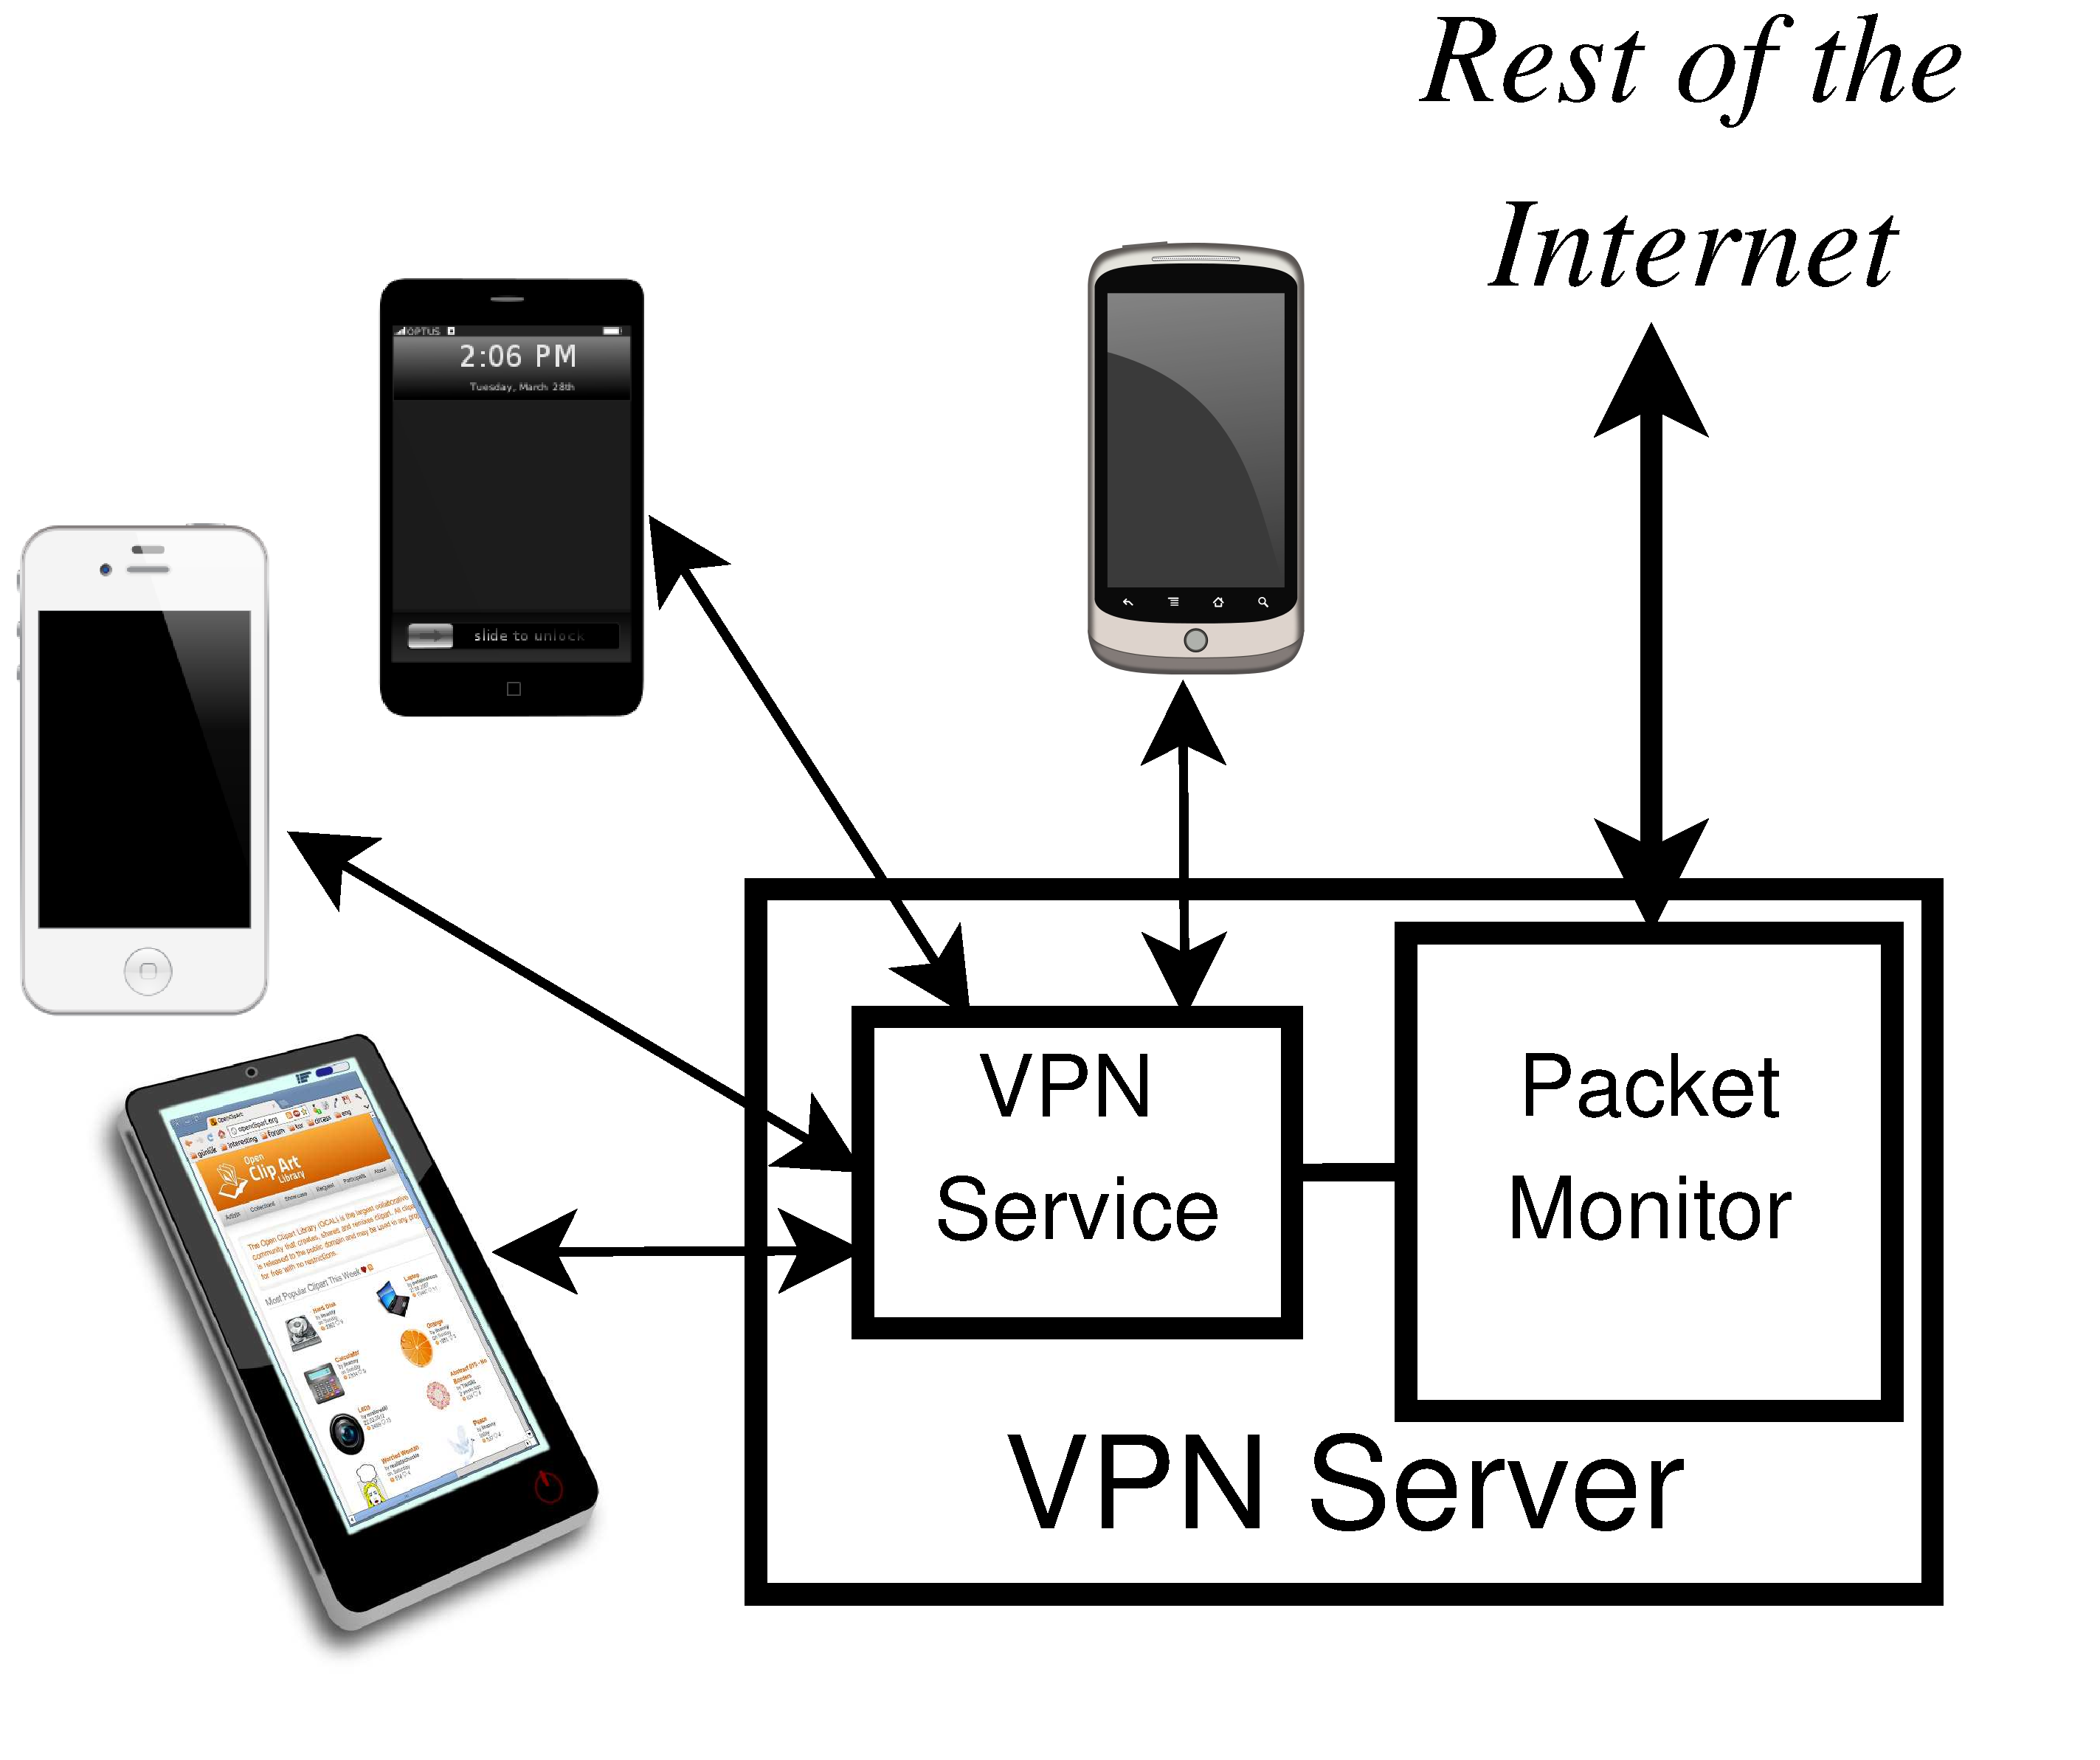
\includegraphics[width=\columnwidth]{figures/meddle-servers.pdf}
\caption{\platname uses traffic proxying to monitor mobile Internet traffic. \platname \emph{requires mobile clients to redirect their traffic through a server that monitors Internet traffic. VPN based proxying is used to characterize mobile traffic sans ISP interference. To detect ISP interference \platname relies on a single hop transparent Web Proxy.}}
\label{fig:description}
\end{figure}

As shown in \fref{fig:description}, mobile devices proxy their Internet traffic through a \platname server that monitors all their Internet traffic. 
%VPNs are used to monitor all Internet traffic from mobile devices while a transparent Web proxy to detail interference by mobile ISPs.
%
%Deploying VPNs on mobile clients is simple for end users primarily VPNs are natively supported by popular mobile OSes. 
%The Android users need to install a certificate and fill our five fields while iOS users need to install a configuration file. 
%Once the configurations are stored, all Internet traffic from the mobile device flows through \platname. 
%\platname uses Strongswan to manage VPN tunnels of \platname.
%This simplicity is important for practical and realistic measurement studies with end users.
We use \emph{tcpdump} to monitor the traffic that passes through \platname servers. We will make the 
configurations and code for \platname public and open source.

Capturing all of a subject's Internet traffic raises significant privacy concerns. Our IRB-approved study 
entails informed consent from subjects who are interviewed in lab, where the risks and benefits of 
our study are clearly explained. Subjects are incentivized to use the VPN though a lottery for Amazon.com 
gift certificates. All data from tcpdump is encrypted before touching persistent storage; the private key 
is maintained on separate secure severs and only approved researchers can access it. Users may 
delete their data and/or disable monitoring at any time. For privacy reasons, we cannot make this 
data publicly available. 



\eat{ Remove text related to tun/tap device
We use tcpdump to monitor the packets that flowing through \platname. 
We now present the technique we used to segregate traffic from mobile devices. 
\platname uses NAT to divert the packets encapsulated in the VPN tunnels to Internet. 
In the ideal scenario, the encapsulated packets from the mobile device would be tunneled to \platname. 
On \platname, these packets would be decapsulated and the packets would then undergo NAT before leaving for their intended destination. 
The packets from the mobile clients to the Internet could be monitored before they undergo NAT.
However, due to the existing network stack implementation, the packets from the Internet that are destined to the mobile clients undergo NAT and IPSec encapsulation take place in one step.
The inter-dependencies between these various modules responsible for routing, NAT, and IPSec make it difficult segregate and monitor the packets. 
We address this issue by looping the packets through a virtual (\emph{tun/tap}) device. 
The looping of packets through a virtual device allows us to monitor the packets when they are outside the VPN tunnels and have not undergone NAT. 
}

\tbd{Dave: \fref {fig:tripnet} text for tripnet should come here}
\begin{figure}
\centering
\tbd{Dave: New figure for Tripnet comes here.} 
\caption{Overview of the Web tripnet }
\label{fig:tripnet}
\end{figure}


%In summary, mobile VPNs are portable and deployable because they are natively supported by popular mobile operating systems.
%We build on existing features provided by iOS and Android to make sure that the VPN tunnels are pervasive and are created passively. 
%We rely on the open source Strongswan VPN daemon to manage VPN tunnels which makes \platname deployable.
%We plan to release the source code to configure mobile Internet traffic using  \platname.

\subsection{Feasibility}

We now show that the cost to proxy traffic through \platname is reasonably low in terms of latency, data consumption, and power.

\subsubsection{VPN Latency Overheads }
The iOS devices use IKEv1 to manage the VPN tunnels while Android devices support both IKEv1 and IKEv2. 
To establish the VPN tunnel, IKEv1 requires a total of 16 packets to be exchanged between the mobile client and the VPN server while IKEv2 requires 4 packets.
\platname uses IKEv2 for Android devices while IKEv1 is used for iOS devices. 

To measure the time required to establish a VPN tunnel, we performed controlled tests using one Android device and an iPhone 5. 
We performed these tests from two different locations based in the same city in which the server was deployed.
OUr tests involved \tbdv{number} of VPN tunnel creation over a time period of \tbdv{} hours. 
When the Android device used \wifi to establish the VPN tunnel, we observe a median connection establishment time of 0.62 seconds from both locations with a maximum of 0.81 seconds and 0.79 seconds respectively. 
When the Android device used cellular networks to establish the tunnel, the median connection establishment time was 0.81 seconds from both locations with a maximum of 1.59 seconds.
Compared to the Android device, the iOS devices required a larger amount of time to establish the connection because it relies on a an older key authentication protocol. 
From the two Wi-Fi networks, to establish the VPN tunnel, the iOS device required 1.60 seconds and 1.34 seconds with a maximum of 2.0 seconds and 1.48 seconds respectively; in the case of cellular networks  we observed a median of 1.80 seconds and 1.65 seconds with a maximum of 2.18 seconds and 1.87 seconds respectively. \drc{This needs to go in a table, since it is impossibly dense.}

\tbd{In summary, we observe that because iOS devices use an older key exchange protocol they can take up to twice as much time as Android devices to establish the VPN tunnel. 
Any more insights .. The tunnel establishment times in the order of 2 seconds implies that \platname can have a significant latency overhead if VPN tunnels are established periodically for short tests.}

\subsubsection{Data Consumption Increase when using VPN}
IPSec encapsulation slightly inflates packet sizes, in addition to preventing carrier middleboxes from applying their own compression.
We measured the overhead of the tunnel in terms of data overhead from IPsec headers and keep-alive messages, finding that it
ranges from 8--12.8\%.

To to compute the increase in the amount of bytes transferred due to encapsulation and the keep-alive
messages, we log the packet lengths of the encrypted packets (IPsec packets) exchanged by our \platname servers and the mobile clients. 
We performed this packet capture for 30 days during which 25 devices tunneled their traffic via \platname. 
During this time interval we also log the packet length of the packets encapsulated within the IPsec packets. 
During this 30 day period we observe that the median of the increase to be 8.31\%, with a maximum increase of 12.8\%.

\tbd{In summary, we observe a maximum overhead of 12.8\% increase in data consumption. We believe the costs of this overhead are minimal compared to the cost of warrant voiding the device.}

\subsubsection{Power Overheads when using VPNs}

We found that VPN proxying imposes approximately 10\% power overhead 
compared to direct traffic. To test the additional power consumption from using a VPN proxy, we used a power meter 
to measure the draw from a Galaxy Nexus running Android 4.2.\footnote{We use Android because power measurements require physical access to 
the battery for a device, which is not feasible for iOS devices. We found similar results when testing the time to discharge 
an iOS device while streaming video with and without a VPN connection.} While instrumented, we conducted 
10-minute experiments where we scripted device usage with and without a VPN 
enabled. The activities included Web searches, map searches, Facebook interaction, 
e-mail and video streaming. 

%
%\subsubsection{Impact of using Transparent Proxy}
%
%\tbd{Dave: Text comes here}

\subsection{Caveats}

Proxying mobile Internet traffic provides a low-cost, portable, pervasive and deployable solution for measurement; however, 
there are several caveats for our approach.

\begin{packedenumerate}
\item When device traffic is proxied, Web sites that use client IP addresses to offer custom services will respond according the IP address of the \platname server. 
\item Some ISPs are known to block VPNs. During our measurement we observed one such ISP that blocked VPN tunnel creation requests from one of our clients.
\item We observe that mobile devices currently create a VPN on at most one wireless interface. This implies that \platname cannot monitor traffic when the mobile device simultaneously uses more than one wireless interface. \drc{Does this ever happen?} 
\item We performed controlled experiments to test IPv6 support. We observe that though iOS and Android support IPv6 they currently do not support IPv6 traffic through VPN tunnels. 
\item When using VPNs, \platname cannot monitor the traffic between the mobile device and access point used to connect to the Internet. \drc{This is unclear to me.}
\end{packedenumerate}

\tbd{In summary, despite these shortcoming we believe that \platname can be used for realistic measurements of mobile Internet traffic.}





